\documentclass{article}
\usepackage{setspace}
\usepackage{gensymb}
\usepackage{xcolor}
\usepackage{caption}
%\usepackage{subcaption}
%\doublespacing
\singlespacing 
%\usepackage{amssymb}
%\usepackage{relsize}
\usepackage[cmex10]{amsmath}
\usepackage{mathtools}
%\usepackage{amsthm}
%\interdisplaylinepenalty=2500
%\savesymbol{iint}
%\usepackage{txfonts}
%\restoresymbol{TXF}{iint}
%\usepackage{wasysym}
\usepackage{amsthm}
\usepackage{mathrsfs}
\usepackage{txfonts}
%\usepackage{stfloats}
\usepackage{float}
\usepackage{cite}
\usepackage{cases}
\usepackage{subfig}
%\usepackage{xtab}
\usepackage{longtable}
\usepackage{multirow}
%\usepackage{algorithm}
%\usepackage{algpseudocode}
\usepackage{enumitem}
\usepackage{mathtools}
%\usepackage{eenrc}
%\usepackage[framemethod=tikz]{mdframed}
\usepackage{listings}
\usepackage{listings} 
\usepackage[latin1]{inputenc} 
%% \usepackage{color} 
%% \usepackage{array} 
%% \usepackage{longtable} 
%% \usepackage{calc} 
%% \usepackage{multirow} 
%% \usepackage{hhline} 
%% \usepackage{ifthen} 
%% %optionally (for landscape tables embedded in another document): 
%% \usepackage{lscape} 
\usepackage{titling}
%\usepackage{fulbigskip}
\usepackage{tikz}
\usepackage{graphicx}
\graphicspath{{/Internal storage/Download/fwc/Figs}}
\begin{document} 
\title{CLASS 9\\10.CIRCLES}
\date{}
\maketitle
\section{EXERCISE 1}
\begin{enumerate}
\item AD is a diameter of a circle and AB is a chord. If AD = 34 cm, AB = 30 cm, the distance of AB from the centre of the circle is:
\begin{enumerate}
\item 17cm
\item 15cm
\item 4cm
\item 8cm
\end{enumerate}
\item In Fig. 10.3, if OA = 5cm, AB = 8cm and OD is perpendicular to AB, then CD is equal to:
\begin{figure}[H]
\centering
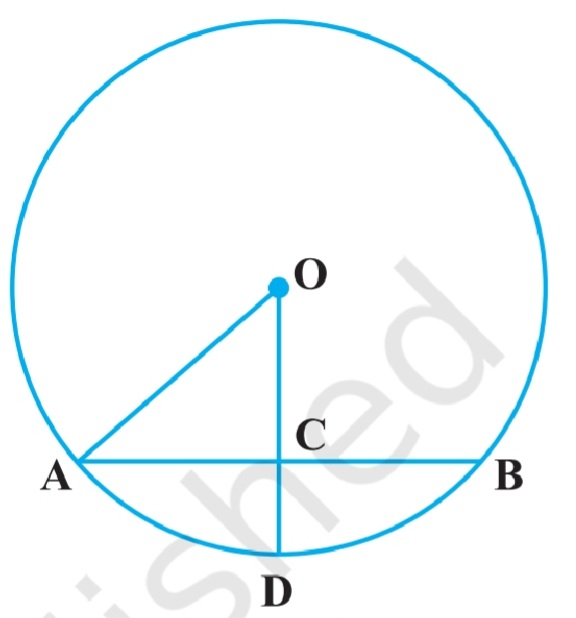
\includegraphics[width=\columnwidth]{Figs/10.3.jpg}
\caption*{Fig:10.3}
\end{figure}
\begin{enumerate}
\item 2cm
\item 3cm
\item 4cm
\item 5cm
\end{enumerate}
\item If AB = 12 cm, BC = 16 cm and AB is perpendicular to BC, then the radius of the circle passing through the points A, B and C is:
\begin{enumerate}
\item 6cm
\item 8cm
\item 10cm
\item 12cm
\end{enumerate}
\item In Fig. 10.4, if $\angle$ ABC = 20$^{\circ}$ , then $\angle$AOC is equal to: 
\begin{figure}[H]
\centering
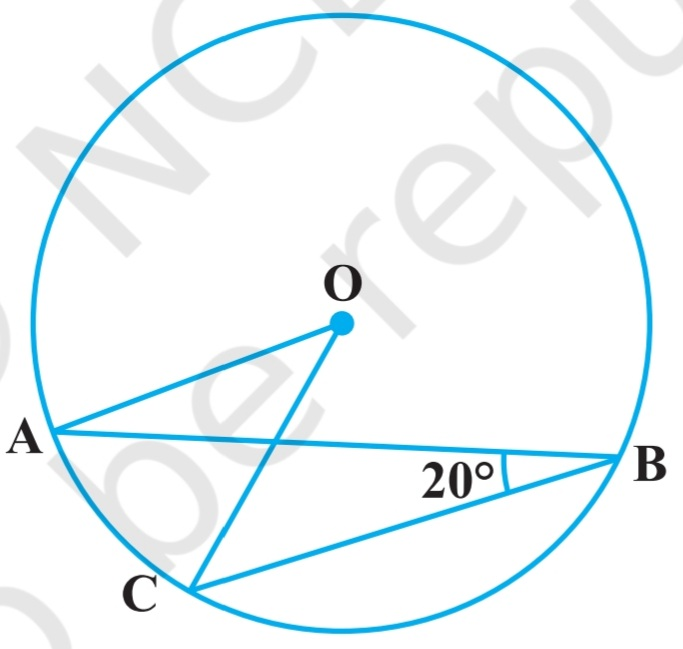
\includegraphics[width=\columnwidth]{Figs/10.4.jpg}
\caption*{Fig:10.4}
\end{figure}
\begin{enumerate}
\item 20$^{\circ}$
\item 40$^{\circ}$
\item 60$^{\circ}$
\item 10$^{\circ}$
\end{enumerate}
\item In Fig.10.5,if AOB is a diameter of the circle and AC = BC,then $\angle$CAB is equal to:
\begin{figure}[H]
\centering
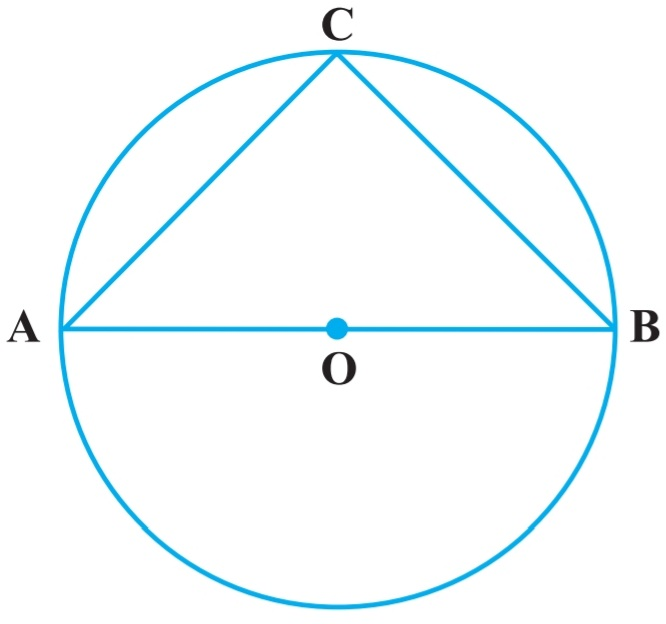
\includegraphics[width=\columnwidth]{Figs/10.5.jpg}
\caption*{Fig:10.5}
\end{figure}
\begin{enumerate}
\item 30$^{\circ}$
\item 60$^{\circ}$
\item 90$^{\circ}$
\item 45$^{\circ}$
\end{enumerate}
\item In Fig. 10.6, if $\angle$OAB = 40$^{\circ}$ , then $\angle$ACB is equal to:             
\begin{figure}[H]
\centering
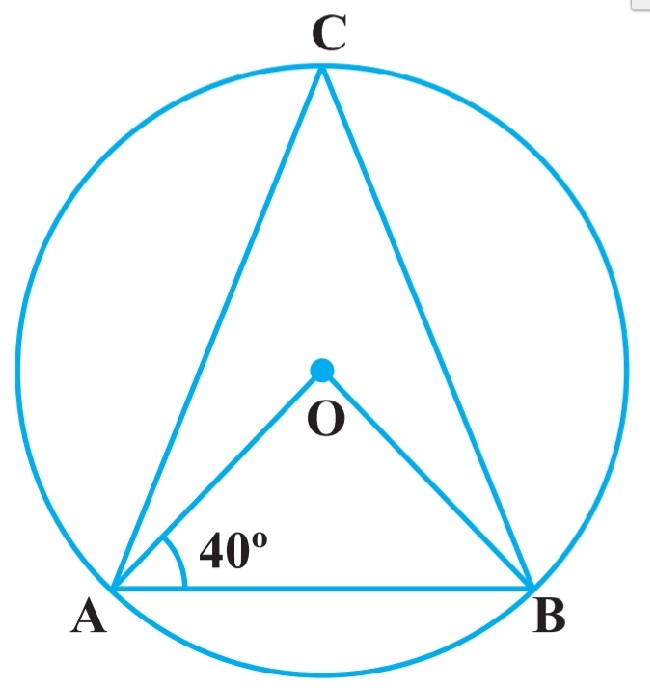
\includegraphics[width=\columnwidth]{Figs/10.6.jpg}
\caption*{Fig:10.6}
\end{figure}
\begin{enumerate}
\item 50$^{\circ}$
\item 40$^{\circ}$
\item 60$^{\circ}$
\item 70$^{\circ}$
\end{enumerate}
\item In Fig. 10.7, if $\angle$DAB = 60$^{\circ}$ , $\angle$ABD = 50$^{\circ}$ , then $\angle$ACB is equal to:
\begin{figure}[H]
\centering
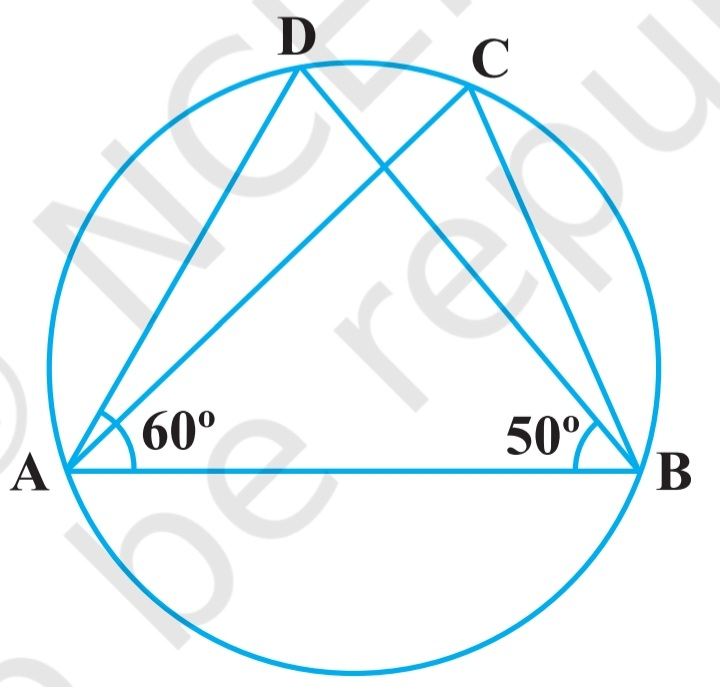
\includegraphics[width=\columnwidth]{Figs/10.7.jpg}
\caption*{Fig:10.7}
\end{figure}
\begin{enumerate}
\item 60$^{\circ}$
\item 50$^{\circ}$
\item 70$^{\circ}$
\item 80$^{\circ}$
\end{enumerate}
\item ABCD is a cyclic quadrilateral such that AB is a diameter of the circle circumscribing it and $\angle$ADC = 140$^{\circ}$ , then $\angle$BAC is equal to:
\begin{enumerate}
\item 80$^{\circ}$
\item 50$^{\circ}$
\item 40$^{\circ}$
\item 30$^{\circ}$
\end{enumerate}
\item In Fig. 10.8, BC is a diameter of the circle and $\angle$BAO = 60$^{\circ}$. Then $\angle$ADC is equal to:
\begin{figure}[H]
\centering
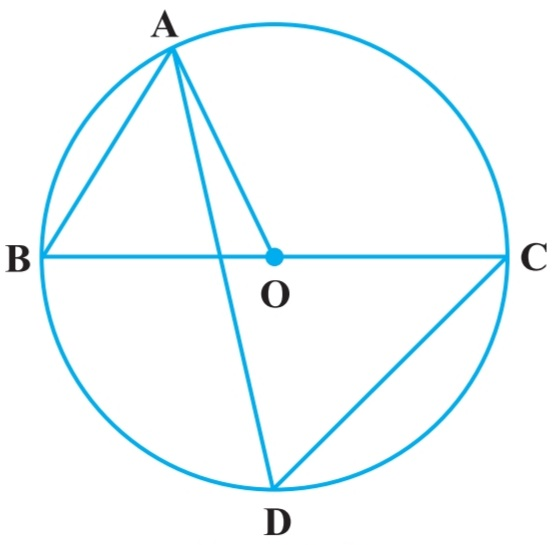
\includegraphics[width=\columnwidth]{Figs/10.8.jpg}
\caption*{Fig:10.8}
\end{figure}
\begin{enumerate}
\item 30$^{\circ}$
\item 45$^{\circ}$
\item 60$^{\circ}$
\item 120$^{\circ}$
\end{enumerate}
\item In Fig. 10.9, $\angle$AOB = 90$^{\circ}$ and $\angle$ABC = 30$^{\circ}$ , then $\angle$CAO is equal to:                              
\begin{figure}[H]
\centering
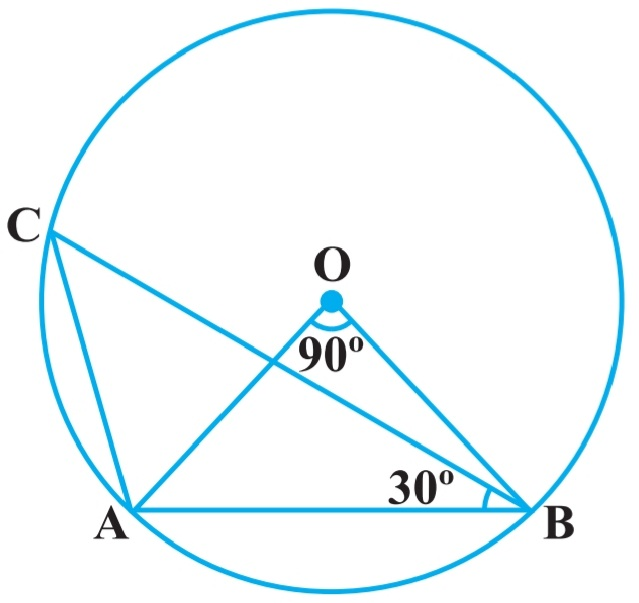
\includegraphics[width=\columnwidth]{Figs/10.9.jpg}
\caption*{Fig:10.9}
\end{figure}
\begin{enumerate}
\item 30$^{\circ}$
\item 45$^{\circ}$
\item 90$^{\circ}$
\item 60$^{\circ}$
\end{enumerate}
\end{enumerate}
\end{document}
